
\section{Daubechies wavelets}
\label{sec:dau}
We now have seen three different bases to represent signals: in the sample domain, in the Fourier domain and in the Haar wavelets domain. They all have different properties. We have reasoned that the Haar wavelets have nice properties regarding images; it is able to represent edges well and errors are local. However a little bit of smoothness is sometimes asked for, this is exactly what the Daubechies wavelets of order four add.

Instead of explicitly defining or showing the basis elements, we will directly describe the wavelet transform $W$.\footnote{Note that we didn't describe the actual transforms described in section~\ref{sec:intro}, as this section was motivational only.} We will describe the transform in terms of matrices, just as in \cite{numc} and \cite{biss}.


\subsection{The Daubechies wavelet transform}
Before we begin with the matrix, we define the following constants:
\begin{align*}
	c_0 &= \frac{1 + \sqrt{3}}{4 \sqrt{2}}, &\quad
	c_1 &= \frac{3 + \sqrt{3}}{4 \sqrt{2}}, \\
	c_2 &= \frac{3 - \sqrt{3}}{4 \sqrt{2}}, &\quad
	c_3 &= \frac{1 - \sqrt{3}}{4 \sqrt{2}}.
\end{align*}

Now let $n$ be even, define the $n \times (n+2)$-matrix $W_n$ as follows (where a blank means $0$).
\[ W_n =
\begin{pmatrix}
	c_0 &  c_1 & c_2 &  c_3 &     &      & & & & & & & \\
	c_3 & -c_2 & c_1 & -c_0 &     &      & & & & & & & \\
	    &      & c_0 &  c_1 & c_2 &  c_3 & & & & & & & \\
	    &      & c_3 & -c_2 & c_1 & -c_0 & & & & & & & \\

	& & & & & & \ddots & & & & & & \\

	& & & & & & & c_0 &  c_1 & c_2 &  c_3 &     &      \\
	& & & & & & & c_3 & -c_2 & c_1 & -c_0 &     &      \\
	& & & & & & &     &      & c_0 &  c_1 & c_2 &  c_3 \\
	& & & & & & &     &      & c_3 & -c_2 & c_1 & -c_0
\end{pmatrix} \]

We also need the \emph{even-odd sort matrix} $S_n$, defined by
\[ (S_n \vec{x})_i = \begin{cases}
	x_{2i}         &\mbox{ if } i  <   \frac{n}{2} \\
	x_{2i - n + 1} &\mbox{ if } i \geq \frac{n}{2},
\end{cases}\]
which permutates the elements of $x$ by putting the elements with an even index in front.

In many cases we want to apply the $n \times (n+2)$-matrix $W_n$ to a vector of length $n$, in order to do so we can set $x_n = x_0$ and $x_{n+1} = x_1$, i.e. we consider $\vec{x}$ to be \emph{periodic}. More precisely we can define a linear map $P_n$ as follows.
\[ P_n \vec{x} = (x_0, \ldots, x_{n-1}, x_0, x_1) \]
Now applying $W_n$ to the periodic $\vec{x}$ is exactly $W_n P_n \vec{x}$.

The wavelet transform now consists of multiplying the above matrices in a recursive fashion. Given a vector $\vec{x}$ of length $n$, calculate $\vec{x}^{(1)} = S_n W_n P_n \vec{x}$, and recurse on the first halve of $\vec{x}^{(1)}$ using $S_\frac{n}{2}$, $W_\frac{n}{2}$ and $P_\frac{n}{2}$. Repeat this procedure and end with the muliplication of $S_4 W_4 P_4$. More formally the wavelet transform is given by:
\[ W \vec{x} := \diag(S_4 W_4 P_4, I_4, \ldots, I_4) \cdots
             \diag(S_\frac{n}{2} W_\frac{n}{2} P_\frac{n}{2}, I_\frac{n}{2})
             S_n W_n P_n \vec{x}. \]


\subsection{The inverse}
Just as the Fourier transform, the wavelet transform is invertible. This makes it possible to go to the wavelet transform, apply some operation and go back. We will proof invertibility of $W$ by first showing that $S_n$ and $W_n P_n$ are invertible. In fact, they are orthogonal, which means that the inverse is given by the transpose.

\begin{lemma}
	The matrices $S_n$ and $W_n P_n$ are orthogonal.
\end{lemma}
\begin{proof}
	For $S_n$ it is clear, as it is an permutation matrix.

	For $W_n P_n$ we should calculate the inner products of all pairs of rows (or columns). If we take the same row, their inner product is:
	\[ c_0^2 + c_1^2 + c_2^2 + c_3^2 = \frac{1}{32}(1 + 3 + 2\sqrt(3)) + 9 + 3 + 6\sqrt(3) + 9 + 3 - 6\sqrt(3) + 1 + 3 -2\sqrt(3)) = 1 \]
	For two different rows we get four non-trivial combinations:
	\begin{align*}
		c_0c_3 - c_1c_2 + c_1c_2 - c_0c_3 &= 0, \\
		c_0c_2 + c_1c_3 &= \frac{1}{32}(3+2\sqrt(3)-3+3-2\sqrt(3)-3) = 0, \\
		c_2c_3 - c_3c_2 &= 0, \\
		c_1c_0 - c_0c_1 &= 0.
	\end{align*}
	For $W_4 P_4$ there is another combination, which can be shown to be zero with a similar calculation. So indeed $W_n P_n (W_n P_n)^T = I_n$.
\end{proof}

\begin{theorem}
	The matrix $W$ is invertible with $W^{-1} = W^T$.
\end{theorem}
\begin{proof}
	Using the fact that the composition of two orthogonal maps is again orthogonal, we easily see that $S_m W_m P_m$ is orthogonal for all even $m$. As a consequence $\diag(S_m W_m P_m, I_m, \ldots, I_m)$ is also orthogonal, and again by multiplication $W$ is orthogonal.
\end{proof}


\subsection{In place}
When implementing this transform, we don't have to perform the even-odd sort. Instead, we can simply do all calculations in place and use a stride to skip the odd elements in further steps. This is depicted in figure~\ref{fig:wavelet_stride}. The only difference with the actual transform $W \vec{x}$ is that the output is permuted. However, in our application of image compression, we are not interested in the index of a coefficient, so we don't need to rectify this. In the rest of this paper the Daubechies wavelet transform will refer to this (in-place) variant.

\tikzstyle{plain_line}=[]
\begin{figure}
	\begin{tabular}{c|c}
	\begin{subfigure}[b]{0.5\textwidth}
		\centering
		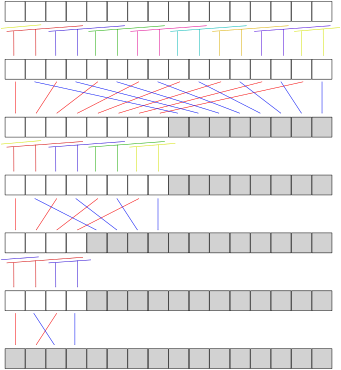
\includegraphics[width=\textwidth]{wavelet_perm}
		\caption{The wavelet transform with the even-odd sort}
	\end{subfigure}&
	\begin{subfigure}[b]{0.5\textwidth}
		\centering
		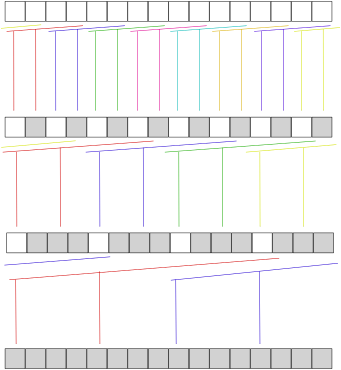
\includegraphics[width=\textwidth]{wavelet_stride}
		\caption{The wavelet transform using a stride to skip odd}
	\end{subfigure}
	\end{tabular}
	\caption{There are two ways to implement the wavelet transform.}
	\label{fig:wavelet_stride}
\end{figure}

Assume we already have a function \texttt{apply\_wn\_pn(x, n, s)} which computes the expression $W_n P_n (x_0, x_s, \ldots, x_{s(n-1)})$ (note the striding) in place\footnote{Implementing this is not so hard, but it would not explain the algorithm better.}. The whole algorithm then can nicely be expressed as

\begin{lstlisting}
for i = 1 to n/4
	apply_wn_pn(x, n/i, i)
	i = i*2
\end{lstlisting}

For future reference we also define the following computation: \texttt{apply\_wn(x, y0, y1, n, s)} which computes $W_n (x_0, \ldots, y_0, y_1)$. Note that \texttt{apply\_wn\_pn(x, n, s)} can now be expressed as \texttt{apply\_wn(x, x0, xs, n, s)}.


\subsection{Costs}
We will briefly analyze the cost of the transform by counting the number of \emph{flops}, that is muliplications and additions. Computing one element of $W_n \vec{x}$ costs $4$ multiplications and $3$ additions. So $W_n \vec{x}$ costs $7n$ flops. Applying  $P_n$ does not require any flops, as is is a mere data manipulation. Consequently computing $W \vec{x}$ costs
\[ 7 \times n + 7 \times \frac{n}{2} + \cdots +  7 \times 8 + 7 \times 4 \text{ flops }. \]
Using the geometric series $\sum_{i=0}^\infty 2^{-i} = 2$ we can bound the number of flops by $14n$.

Compared to the FFT this is a big improvement in terms of scalability, as this wavelet transform has a linear complexity $\BigO{n}$, but the FFT has a complexity of $\BigO{n \log n}$. This is however also a burden, as it leaves not much room for overhead induced by parallelizing the algorithm: the sequential version takes $14n$ flops and the parallel version at best $14\frac{n}{p}$ flops, where $p$ is the number of processors. So we see that the communication overhead may not exceed $14(p-1)\frac{n}{p}$ flops.


\subsection{Higher dimensional wavelet transform}
Our final goal is to apply the wavelet transform to images. Of course we could simply put all the pixels of an image in a row and apply $W$. But if we do this, we don't use the spatial information of the image at all! In order to use the spatial information we have to apply $W$ in both directions. To be precise: we will apply $W$ to every row and then apply $W$ to all of the resulting columns. We can also do this the other way around, but this does not matter:

\begin{notation}
	Given a $n \times n$-matrix $F$ and an $m \times n$-matrix $X$ (which should be thought of as an image). Applying $F$ to each row of $X$ individually is denoted as $F^{H} X$.
	Given a $m \times m$-matrix $G$, then appling $G$ on the columns of $X$ is denoted by $G^{V} X$.
\end{notation}
\begin{lemma}
	Given a $n \times n$-matrix $F$ and a $m \times m$-matrix $G$ and an $m \times n$-matrix $X$, then $G^{V}(F^{H} X) = F^{H}(G^{V} X)$.
\end{lemma}
\begin{proof}
	This can be done by writing out all matrix multiplication and then interchanging the sums and using commutativity of multiplication of reals. We left out the calculation for brevity.
\end{proof}

This lemma expresses some sort of commutativity and generalises to higher dimensions by apply this commutativity inductively. As we don't need the general statement (i.e. we will only apply $W$ to images) we won't spell out the proof. If we say that we apply $W$ to an image, it is meant that we actually apply $W^{H} W^{V}$. On non-square images we also use this notation, despite the fact that the first $W$ has a different size than the second.
